\documentclass[12pt]{article}
\usepackage{amsmath}
\usepackage{amsfonts}
\usepackage{float}
\usepackage{graphicx}
\usepackage{hyperref}
\usepackage{tikz}
\usetikzlibrary{shapes.geometric}
\usepackage{listings}
\usepackage{algorithm}
\usepackage{algorithmic}
\usepackage[margin=0.6in]{geometry}

\title{OCNN FPGA Implementation: Sparse 3D Convolution with Hierarchical Bitmap Compression}
\author{Chenhe Yuan}
\date{\today}

\begin{document}

\maketitle

\section{Scenario Setting}

We're dealing with sparse 3D voxel data - a 3D grid where most cells are empty and only some cells contain actual objects. This could be from a 3D sensor scanning a room, or medical imaging data, or any 3D scene where there's a lot of empty space.

The problem is that regular 3D convolution treats every single voxel the same way, spending tons of computation and memory on empty regions that don't contribute anything meaningful. We want to build a system that only processes the parts that actually matter - the non-empty voxels - while still being able to find neighbors for convolution operations.

The whole system runs on FPGA hardware, processing this sparse 3D data in a streaming fashion where voxel data comes in continuously and we process the data on-the-fly, and perform 3D convolutions efficiently.

\section{Core Concepts}

\subsection{Morton Code Properties}
Morton codes (Z-order) take 3D coordinates (x,y,z) and create a single number by interleaving their binary representations. The key property we care about is that spatially close points get numerically similar Morton codes.

For example, if you have points (2,3,1) and (2,3,2), their Morton codes will be very close numerically. But a distant point like (7,1,6) will have very different Morton code.

This is great for DRAM because accessing similar addresses is much faster due to row buffer behavior - you get hits instead of misses. But it creates a several conflict in our system: Our bitmap structure requires sequential access through access pointers, but Morton ordering creates a random access pattern.

\subsection{Hierarchical Bitmap}

A big 3D cube of voxels, and we create multiple "zoom levels" of this cube:

\begin{itemize}
    \item \textbf{L0 (original data):} Your full resolution voxel grid
    \item \textbf{L1:} Divide the L0 cube into 2×2×2 (=8) blocks. Each bit in L1 represents one of these 8-voxel blocks
    \item \textbf{L2:} Take L1 and divide it into groups of 8 bits like we did in L1. Each bit in L2 represents 8 L1 bits, which means 8 $\times$ 8 = 64 L0 voxels
    \item \textbf{L3 and higher:} Keep going with the same pattern
\end{itemize}

The encoding rule is that if a region has ANY non-empty voxels, the bit is 1. If the entire region is completely empty, the bit is 0.

If a higher level bit is 0, we know for certain that everything below it is empty, so we don't store those lower-level bits at all. We just skip them entirely. One empty bit in L3 means 8 empty bits in L2 and thus 64 empty bits in L1 and thus 512 empty voxels in the sparse space.

\section{Key Components and Data Flow}

Voxel data comes in from the sensor through the PS interface. The first place it arrives at is the bitmap generator, which is doing two jobs simultaneously - it's figuring out which regions are empty or not empty to build our hierarchical bitmap, and it's also buffering the actual feature data that we'll need later.

The bitmap gets stored in BRAM because we need fast access to it. The feature data, meanwhile, gets sent to a Morton reorder buffer. This buffer sorts the memory write requests based on their Morton codes before sending them to DRAM, because we want to get row bufer hits.

And the systolic array doesn't wait for the entire frame to finish. As soon as there's enough data available, it starts processing. The controller reads the bitmaps from BRAM to figure out where the actual data is stored, calculates the DRAM addresses, and sends read requests through another Morton reorder buffer. But we need to properly control how the systolic array knows when it can start reading from DRAM.

The tricky part is the neighbor finding. For 3D convolution, each voxel needs to look at its 26 neighbors in a 3×3×3 cube. But our data is stored in this compressed format that you can only access sequentially. That's where the 3-layer Z-buffer comes in, which I'll explain in detail later.

Finally, the systolic array does the actual convolution math and writes results back to DRAM through the Morton reorder system.

\section{Hierarchical Bitmap Compression}

\subsection{How to Divide the Space}

At the bottom (L0), you have your original voxel data at full resolution. But each level above represents larger and larger chunks of space.

L1 takes every 2×2×2 cube from L0 and asks: "Is there anything here?" If yes, the bit is 1. If the entire 2×2×2 cube is empty, the bit is 0.

L2 does the same thing but for groups of 8 L1 bits. So one L2 bit actually represents a much larger region - equivalent to a 4×4×4 cube in the original L0 space.

This keeps going up the pyramid until you reach the top level, which might only have 8 bits total.

\subsection{What We Skip}

If any bit is 0, we know that everything below it in the hierarchy is definitely empty. So we don't store those lower-level bits at all.

Let's say L2 looks like: [1, 0, 1, 0]. This tells us:
- Region 0: Has some data, so we need to store the corresponding 8 L1 bits
- Region 1: Completely empty, so we skip storing its 8 L1 bits entirely
- Region 2: Has some data, so we store its 8 L1 bits  
- Region 3: Completely empty, skip it

For the regions we do store in L1, we apply the same logic going down to L0.

\subsection{Streaming Construction Algorithm}

\begin{algorithm}
\caption{Hierarchical Bitmap Construction}
\begin{algorithmic}
\REQUIRE Incoming voxel data stream in scanline order
\ENSURE Hierarchical bitmap with pruned storage

\STATE Initialize small-block buffer for 2 Z-layers
\STATE Initialize bitmap levels L0, L1, L2, ...

\WHILE{voxel data available}
    \STATE Buffer incoming 2×2×2 voxel blocks
    
    \IF{all 8 bits in block are zero}
        \STATE Set corresponding L1 bit = 0
        \STATE Do not store this L0 block
    \ELSE
        \STATE Set corresponding L1 bit = 1
        \STATE Store this L0 block in memory
    \ENDIF
    
    \IF{8 consecutive L1 bits ready}
        \IF{all 8 L1 bits are zero}
            \STATE Set corresponding L2 bit = 0
            \STATE Do not store these L1 bits
        \ELSE
            \STATE Set corresponding L2 bit = 1
            \STATE Store these L1 bits
        \ENDIF
    \ENDIF
    
    \STATE Continue for higher levels as needed
\ENDWHILE
\end{algorithmic}
\end{algorithm}

\section{Access Pointer Mechanism}

Since we've skipped storing empty regions, the data isn't in nice continuous blocks anymore. We need a way to navigate through this compressed structure and figure out where the actual data is located.

We maintain access pointers for each level that track where we are in the stored data. The reconstruction works by starting at the top level and working downward. When we encounter a 0 bit, we know to skip ahead without accessing any storage. When we encounter a 1 bit, we know there's actual data to read at the lower levels.

\subsection{Access Algorithm}

\begin{algorithm}
\caption{Bitmap Access and Reconstruction}
\begin{algorithmic}
\REQUIRE Hierarchical pruned bitmap, access pointers for each level
\ENSURE Sequential access to non-empty voxel regions

\STATE Initialize pointers: current\_ptr\_L1, current\_ptr\_L0
\STATE Start at top level (L2)

\FOR{each bit in L2}
    \IF{L2[bit] == 0}
        \STATE Skip entire corresponding L1 block
    \ELSE
        \STATE Access L1 block via current\_ptr\_L1
        
        \FOR{each bit in accessed L1 block}
            \IF{L1[bit] == 0}
                \STATE Skip corresponding L0 block
            \ELSE
                \STATE Access L0 block via current\_ptr\_L0
                \STATE Process actual voxel data
                \STATE Increment current\_ptr\_L0
            \ENDIF
        \ENDFOR
        
        \STATE Increment current\_ptr\_L1
    \ENDIF
\ENDFOR
\end{algorithmic}
\end{algorithm}

\subsection{Key Properties}
\begin{itemize}
    \item \textbf{Sequential-only access:} Pointers can only move forward, no random access (and thus can't access 26 neighbors of a center voxel easily)
    \item \textbf{Deterministic reconstruction:} Given bitmap structure, reconstruction is completely predictable
    \item \textbf{Massive skip capability:} Can skip large empty regions without any data access
\end{itemize}

\section{Morton Reordering}

The Morton reorder buffer collects memory requests along with their Morton codes, sorts them numerically, then sends them to DRAM in that order. This should improve DRAM performance because accessing nearby addresses (in the same row) is much faster than jumping around randomly.

The sorting can be done with a simple sorting network since we're dealing with a bounded number of requests at a time.

\section{3-Layer Z-Buffer Neighbor Finding Algorithm}

\subsection{The Core Problem}

We need to do 3D convolution, which requires looking at 3×3×3 neighborhoods around each voxel. That's 27 neighbors for every voxel. But our data is stored in this compressed bitmap format that only allows sequential access through access pointers.

Traditional approaches fail here. You could search through the entire dataset for each neighbor (O(N²) complexity), or try to build hash tables, but that defeats the purpose of compression.

\subsection{The Key Insight}

Any 3×3×3 convolution kernel spans exactly 3 consecutive Z layers. If we buffer these 3 complete Z layers in memory, then every voxel in the middle layer is guaranteed to have all its 27 neighbors available locally.

\subsection{How It Works}

For each Z position (center voxel's z-coordinate):
1. Load the next Z layer using our expensive sequential access pointers (not that expensive when we read sequentially, we can read 3 layers of bits and this is just one long run, it's just reusing the reconstructed bit)
2. Process all voxels (as center voxels) in the current middle layer (all neighbors are guaranteed to be in the 3-layer buffer)
3. Slide the buffer window forward and repeat

\subsection{Algorithm}

\begin{algorithm}[H]
\caption{3-Layer Z-Buffer Streaming Convolution}
\begin{algorithmic}
\REQUIRE Hierarchical bitmap, DRAM feature storage
\ENSURE 3D convolution results for all valid voxels

\STATE Allocate 3-layer buffer: layer[3][max\_voxels\_per\_layer]
\STATE Initialize access pointers to pruned bitmap
\STATE Set current\_z = 1

\FOR{Z = 1 to (DIM\_L0 - 2)}
    
    \STATE Use access pointers to read layer Z+1 from pruned bitmap
    \STATE Store voxel locations and Morton codes in buffer[2]
    
    \FOR{each voxel V in buffer[1]}
        
        \FOR{each of 27 neighbor offsets}
            \STATE Calculate neighbor coordinates (x±1, y±1, z±1)
            \STATE Look up neighbor in appropriate buffer layer [0,1,2]
        \ENDFOR
        
        \STATE Read feature values from DRAM for non-empty neighbors
        \STATE Execute convolution: weights × features + bias
        \STATE Apply activation function
        \STATE Store result to output buffer
        
    \ENDFOR
    
    \STATE buffer[0] = buffer[1]
    \STATE buffer[1] = buffer[2] 
    \STATE buffer[2] = empty
    \STATE Increment current\_z
    
\ENDFOR
\end{algorithmic}
\end{algorithm}

\subsection{Complexity Improvement}

This transforms the problem from O(N²) to O(N). Each voxel and each layer gets processed exactly once. The expensive sequential access through the bitmap only happens once per Z layer instead of once per neighbor lookup.

\section{Memory Arrangement and Management}

The system has to carefully manage different types of memory accesses to avoid conflicts:

\textbf{BRAM Usage:}
- Hierarchical bitmaps are stored in BRAM for fast access
- 3-layer Z-buffer uses BRAM for storing voxel locations and Morton indices
- Different pipeline stages must use different BRAM address ranges

\textbf{DRAM Usage:}
- Feature data is written to DRAM in Morton-ordered addresses
- Same DRAM addresses are later read for convolution processing
- Results are written to a separate DRAM address range
- All DRAM accesses go through Morton reorder buffers

\textbf{Address Management:}
Different pipeline stages operate on different address ranges:
- Bitmap generation writes to BRAM addresses [A1, B1]
\newline
- Feature retrieval reads the bitmaps from BRAM addresses [A1, B1] but the exact addresses between this and feature writing are different at any given time, write\_address $>$ read\_address
 at any given time
 \newline
- Feature writing in morton stage (which is controlled by bitmap generation stage) uses DRAM range [C1, D1]
\newline
- Feature reading in convolution stage uses the same DRAM range [C1, D1], but the exact addresses between this and feature writing are different at any given time, write\_address $>$ read\_address
 at any given time
 \newline
- Result writing uses separate DRAM range [C2, D2]

\section{Dataflow}
\begin{figure}[htbp]
    \centering
    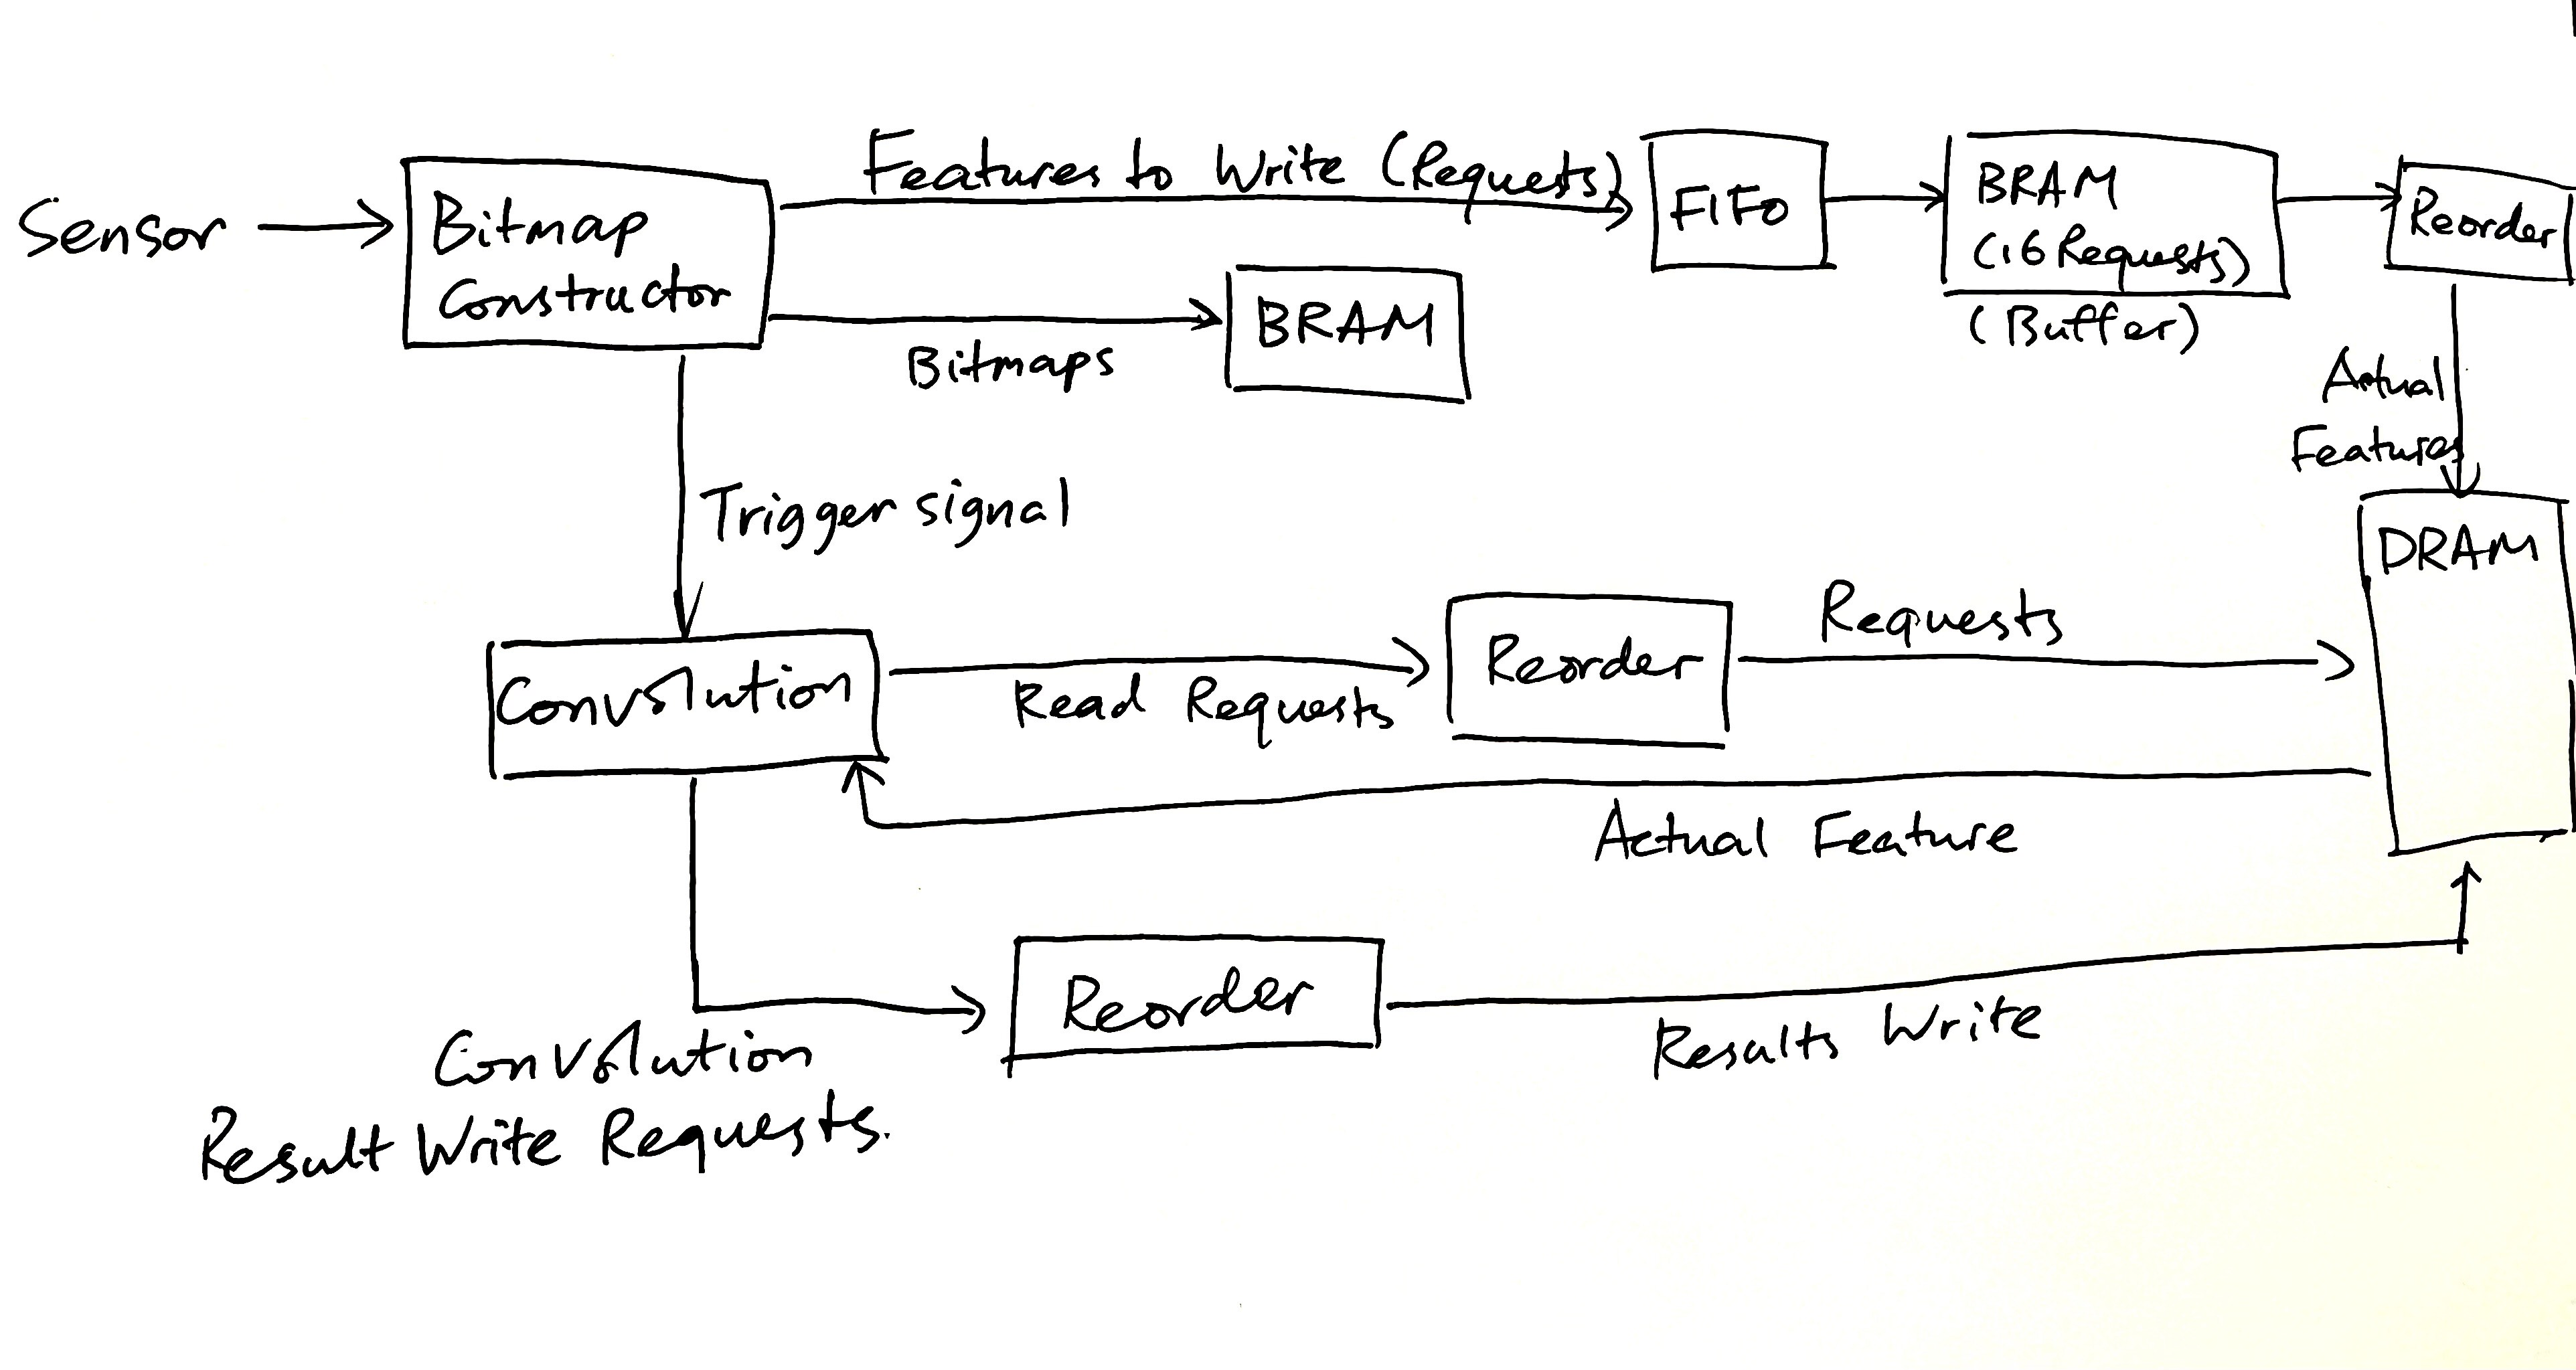
\includegraphics[scale=0.14]{dataflow.jpeg}
    \label{fig:dataflow}
\end{figure}

\end{document}